\documentclass{standalone}
\usepackage{tikz}
\usetikzlibrary{circuits.logic.US}
%\usetikzlibrary{positioning}

\begin{document}

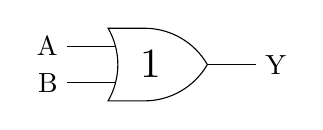
\begin{tikzpicture}[circuit logic US, scale=1.5]
	 \node [or gate, inputs=nnn] (lg1) {1};
	 \draw (lg1.input 1) -- node[at end,left]{A} ++(left:4mm);
	 \draw (lg1.input 3) -- node[at end,left]{B} ++(left:4mm);
	 \draw (lg1.output) -- node[at end,right]{Y} ++(right:4mm);
 \end{tikzpicture}

\end{document}